% !TeX spellcheck = cs_CZ
%{\tikzset{external/prefix={tikz/CES/}}
% \tikzset{external/figure name/.add={ch05_}{}}
%---------------------------------------------------------------------------------------------------
% file ANSI_C_MCU.tex
%---------------------------------------------------------------------------------------------------
%============================= Kapitola: Stručný úvod===============================================
\lstset{ %
  language=C,                            % choose the language of the code
  basicstyle=\fontsize{9}{11}\ttfamily,  % the size of the fonts that are used for the code
  backgroundcolor=\color{beige},         % choose the background color. 
  commentstyle=\color{cadmiumgreen}\textit,
  keywordstyle=\color{blue(pigment)}\textbf,
  breaklines=true,                       % sets automatic line breaking
  breakatwhitespace=true,                % sets if automatic breaks should only happen at whitespace
  showspaces=false,                      % show spaces adding particular underscores
  showstringspaces=true,                 % underline spaces within strings
  showtabs=true,                         % show tabs within strings adding particular underscores
  frameround = ffff,
  frame=trBL,                            % adds a frame around the code - none, single
  rulesepcolor=\color{bazaar},
  tabsize=2,                             % sets default tabsize to 8 spaces
  captionpos=b,                          % sets the caption-position to bottom
  numbers=left,                          % where to put the line-numbers -none, left, right
  numberstyle=\tiny,                     % the size of the fonts that are used for the line-numbers
  stepnumber=1,                          % the step between two line-numbers. If it's 1 each line
  % will be numbered
  xleftmargin=3em,                       % adjust left margin
  xrightmargin=6em,                      % adjust right margin
  rulecolor=\color{black},               % rule 
  breaklines=true,
  lineskip=0pt
}

\chapter{Programování vestavěných systémů}
\minitoc
  Tato kapitola demonstruje programování vestavěných systémů s využitím různých nástrojů s 
  otevřeným zdrojovým kódem, včetně sady \wikiGCC (GCC), což je standardní sada překladačů 
  vytvořených v rámci projektu GNU, který je v tomto oboru běžně používán. 
  
%  Each embedded system is unique, and the hardware is highly specialized to the application 
%  domain. As a result, embedded systems programming can be a widely varying experience and can 
%  take years to master. However, one common denominator across almost all embedded software 
%  development is the use of the C programming language. This book will teach you how to use C in 
%  any embedded system.
  
  Každý vestavěný systém je unikátní, což souvisí s tím, že hardware je silně specializovaný pro 
  danou aplikaci. Z toho vyplývá, že programování těchto systémů vyžaduje velké zkušenosti, neboť 
  programátor není odstíněn od hardware. Pokud se zeptáme, co mají tyto systémy společného, pak 
  jednoznačnou odpovědí je, že se programují jazykem \texttt{C}.
  
  V současné době je to jeden z nejpopulárnějších jazyků a to nejen pro aplikace v zabudovaných 
  systémech (viz \ref{chap:ces_arm}), ale zřejmě také je nejčastějším jazykem pro psaní systémového 
  softwaru.
  
  %============= Podkapitola: Základní pojmy =======================================================
  \section{Stručná historie a charakteristika jazyka  C}
    \wikiANSIC vznikl počátkem 70. let 20. století. Jazyk vyvinuli \emph{Ken Thompson} a 
    \emph{Dennis Ritchie} (obr. \ref{ces:fig007}) pro potřeby operačního systému \texttt{Unix}.  
    
    \texttt{C} lze charakterizovat je nízkoúrovňový, kompilovaný, relativně minimalistický 
    programovací jazyk. Je také dostatečně mocný na většinu systémového programování (ovladače a 
    jádro OS), přičemž zbytek lze dořešit tzv. \wikiInlineASM, tedy metodou zápisu assembleru přímo 
    do kódu. Zdrojový kód \texttt{C} je přitom mnohem čitelnější než assembler, je jednodušší ho 
    zapsat a navíc je daleko snáze přenositelný na jiné procesory a počítačové architektury. Proto 
    jsou často operační systémy, překladače, knihovny a interprety vysokoúrovňových jazyků 
    implementovány právě v \texttt{C}. 
    
    Mnoho dalších moderních programovacích jazyků přebírá způsob zápisu (neboli syntaxi) z jazyka 
    \texttt{C}, například \wikiCPP, Java, Perl a PHP.
  
    \begin{figure}[ht!]  %\ref{ces:fig007}
      \centering
      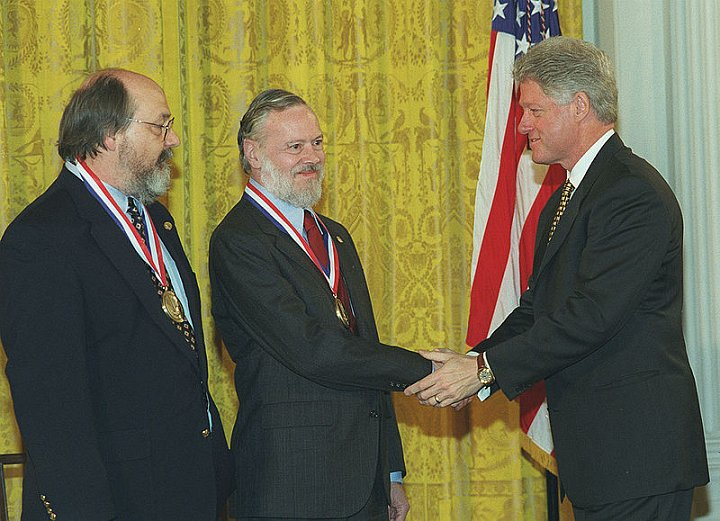
\includegraphics[width=0.5\linewidth]{ces_fig007.jpg}
      \caption{Autoři jazyka \texttt{C} Ken Thompson a Dennis Ritchie přebírají ocenění v podobě 
               Národní medaile za technologii (v roce 1998) od Billa Clintona}
      \label{ces:fig007}
    \end{figure}
    
    V roce 1973 se stal jazyk \texttt{C} dostatečně stabilním. Proto většina zdrojového kódu jádra 
    \texttt{Unixu}, původně napsaného v assembleru, byla přepsána do \texttt{C}. \texttt{Unix} tedy 
    patří mezi první operační systémy, které byly napsané v jiném než strojovém jazyce či 
    assembleru. To také přispělo k velké popularitě tohoho jazyka. 
    
    V roce 1978, Ritchie a Brian Kernighan vydali famózní knihu \emph{The C Programming Language}. 
    Tato kniha, mezi programátory \texttt{C} známá jako „K\&R“, sloužila po mnoho let jako 
    neformální specifikace jazyka. Verze C, kterou takto popsali, bývá označována jako 
    „\textbf{K\&R C}\footnote{Druhé vydání knihy popisovalo novější standard \texttt{ANSI C}.}“.
                        
    Dalšími milníky vývoje jazyka \texttt{C} jsou dány standardizačnímy procesy organizace American 
    National Standards Institute (ANSI) a International Organization for Standardization ISO:
    \begin{description}
      \item[C89]    V roce 1983 se \texttt{ANSI} dohodla na sestavení komise, aby vytvořila 
                    standardní specifikaci C. Po dlouhém procesu byl standard dokončen v roce 1989 
                    a schválen jako ANSI X3.159-1989 „\emph{Programming Language C}“. Tato verze 
                    jazyka je často stále označována jako \textbf{ANSI C} nebo \textbf{C89}.
      \item[C90]    V roce 1990 byl standard ANSI C (s drobnými změnami) adoptován institucí ISO 
                    jako „ISO 9899|ISO/IEC 9899:1990“. Formálně tak nahradil předchozí verzi 
                    C89/ANSI-C a tato revize je označována jako \textbf{C90} neboli \uv{jazyk C}. 
                    Technicky je to stejný standard jako C89/ANSI-C.
      \item[C99]    Po standardizaci jazyka v roce 1989 - 1990 se většina vývoje soustředila na 
                    jazyk \texttt{C++}. Přesto však na konci 90. let došlo k vydání dokumentu ISO 
                    9899:1999 (obvykle nazývaný \textbf{C99}), který byl následně v březnu 2000 
                    přijat i jako ANSI standard. C99 představil několik nových vlastností, které 
                    byly mnohdy v překladačích už dávno implementovány jako rozšíření.
      \item[C11]    V roce 2007 začala práce na další revizi standardu \texttt{C}, neformálně 
                    nazývaného "C1X", až do oficiálního zveřejnění dne 2011-12-08. Výbor pro 
                    standardy \texttt{C} přijal pokyny, které omezují přijetí nových funkcí, které 
                    nebyly testovány stávajícími implementacemi.
    \end{description}
    
    \begin{note}
      První norma pro \texttt{C} byla tedy vydána společností ANSI. Ačkoli tento dokument byl 
      následně přijat Mezinárodní organizací pro normalizaci (ISO) a následné revize vydané 
      společností ISO byly také přijaty ANSI, mnozí programátoři stále používají "\emph{ANSI C}", 
      ačkoliv se odkazují na ISO standard. Jiní vývojáři softwaru používají termín \emph{ISO C}, 
      ostatní jsou neutrální a používají \emph{Standard C}.
    \end{note}
  
  \newpage
  %============= Podkapitola: Základní pojmy =======================================================
  \section{Základní pojmy}
    \subsection{Způsob zpracování C programu}
      Chceme-li jazyk C opravdu využívat, je nutné seznámit se i trochu více s tím, jak se program 
      vlastné zpracovåvå, od napsåni zdrojového text až po spuštění přeloženého a sestaveného 
      programu.
      
      Zåkladni zpracovåni programu v \texttt{C} probíhá několika fázemi schematicky vyjádřenými 
      nåsledujicim obråzkem: 

      \begin{figure}[ht!]  %\ref{ces:fig008}
        \centering
        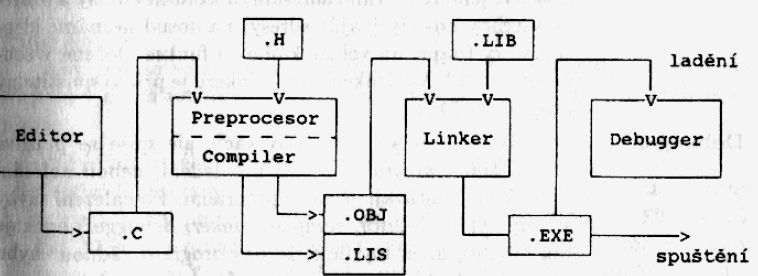
\includegraphics[width=0.7\linewidth]{ces_fig008.png}
        \caption{Zpracování zdrojového textu do podoby spustitelného programu \texttt{EXE}}
        \label{ces:fig008}
      \end{figure}
      
    \subsection{Fixed Width Integers: Sometimes Size Matters}
      Programátoři se ne vždy starají o to, jaké paměťové nároky má datový typ \textbf{integer} v 
      mikrokontrolér. Prohlédněme si tento příklad:
      \begin{lstlisting}[gobble=8, xrightmargin=13em]
        int i; 
        
        for (i = 0; i < N; i++) { ... } 
      \end{lstlisting}
      Obecně očekáváme, že překladač (\emph{compilator}) vygeneruje co nejefektivnější kód, a 
      zároveň předpokládámé, že během inkrementace proměnné \texttt{i} smyčkou 
      \lstinline[basicstyle=\ttfamily]!for! nevznikne číslo, které by nešlo uložit do překladačem 
      zvolené paměťové buňky, která může mít velikosti 8, 16, 32 nebo třeba 64 bitů. A to je přesně 
      to, co standardy \texttt{ISO C} a  \texttt{C++} říkají tvůrcům kompilátorů: vybrat 
      nejefektivnější velikost datového typu, která splní konkrétní požadavek. Velikosti celých 
      čísel u různých typů procesorů není pevná. Spolu s odpovídající flexibilitou standardů jazyka 
      \texttt{C}, bude v předchozím kódu proměnná \texttt{i} chápana jako 32bitové nebo 16bitové 
      celé číslo v závislosti na použitém překladači a to i v případě, že cílový (\emph{target}) 
      mikrokontrolér stejný.
      
      V mnoha ostatních situací, ovšem na velikosti datového typu integer záleží \(\Rightarrow\) 
      \textbf{Embedded programming}. 
      
      But in many other programming situations, integer size matters. Embedded programming, in 
      particular, often involves considerable manipulation of integer data of fixed widths. 
      In hindsight, it sure would've been nice if the authors of the C standard had defined some 
      standard names and made compiler providers responsible for providing the appropriate typedef 
      for each fixed-size integer type in a library header file. Alternatively, the C standard 
      could have specified that each of the types short, int, and long has a standard width on all 
      platforms; but that might have had an impact on performance, particularly on 8-bit processors 
      that must implement 16- and 32-bit additions in multi-instruction sequences. 
      Interestingly, it turns out the 1999 update to the International Organization for 
      Standardization's (ISO) C standard (also referred to as C99) did just that. The ISO has 
      finally put the weight of its standard behind a preferred set of names for signed and 
      unsigned fixedsize integer data types. The newly defined type names are: 
      \begin{itemize}
        \item  8-bit: \textbf{int8\_t},  \textbf{uint8\_t}
        \item 16-bit: \textbf{int16\_t}, \textbf{uint16\_t}
        \item 32-bit: \textbf{int32\_t}, \textbf{uint32\_t}
      \end{itemize}
      

  %============= Podkapitola: Konstrukce a struktura programu v jazyce C ===========================
  \section{Konstrukce a struktura programu v jazyce C}
  %============= Podkapitola: Proměnné datové typy, rozsahy platnosti a hodnot =====================
  \section{Proměnné datové typy, rozsahy platnosti a hodnot}
  %============= Podkapitola: Operátory ============================================================
  \section{Operátory}
  %============= Podkapitola: Funkce a práce s pamětí ==============================================
  \section{Operátory}
    \subsection{Bitové  operátory}
      Protože jazyk \texttt{C} je oproti jiným vyšším jazykům zaměřen na přeci jen poněkud nižší 
      úroveň, 
      nabízí programátorům i operátory, pomocí kterých mohou nepřímo pracovat i s jednotlivými bity.
      Tuto možnost zdaleka nemají všechny programovací jazyky označované jako \emph{vyšší}.
      
      Bitové operátory \(<<\), \(>>\), \&, |, \~, \^, tedy posun vlevo, posun vpravo, and, or, not 
      a xor jsou povoleny pouze pro celočíselné (integer) datové typy char, int, short, long (se 
      znaménkem (signed) nebo bez znaménka (unsigned)). V závislosti na MCU a kompilátoru se tyto 
      příkazy převádějí na odpovídající výkonné strojové instrukce. Toto hardwarově blízké bitové 
      řízení často nalézá uplatnění při přístupu na speciální registry v mikrokontroléru. 
      (\cite[s.~79]{Burkhard2003}).
      
      Při bitovém posunu vlevo (vpravo) << , ( >> ) se jednotlivé bity posouvají vlevo (vpravo), 
      tedy do pozice s (binárně) vyšším (nižším) řádem. Na nejpravější (nejlevější) posunem 
      vytvořenou pozici je umístěna nula. Posuny ovšem probíhají aritmeticky. To znamená, že 
      uvedené pravidlo neplatí pro posun vpravo hodnoty celočíselného typu se znaménkem. V takovém 
      případě se nejvyšší bit (znaménkový), zachovává. Takto se při posunu doplňuje do bitového 
      řetězce nový bit. Naopak před posunem nejlevější (nejpravější) bit je odeslán do
      "říše zapomnění.
      
      Bitový posun o jeden (binární) řád vpravo, respektive vlevo, má stejný význam, jako 
      celočíselné dělení, respektive násobení, dvěma. Je-li bitový posun o více než jeden řád, 
      jedná se o násobení (dělění) příslušnou mocninou dvou.
      
      Bitové and \& , or |, a xor \^ provádí příslušnou binární operaci s každým párem 
      odpovídajících si bitů. Výsledek je umístěn do pozice stejného binárního řádu výsledku. 
      Výsledky operací nad jednotlivými bity jsou  stejné, jako v Booleově algebře9. Bitové not \~ 
      je operátorem unárním, provádí negaci každého bitu v bitovém řetězci jediného operandu. 
      Tomuto operátoru se často říká bitový doplněk. 
      
      \subsubsection{Makra pro bitové operace}
        O něco elegantnější je použití maker k nahazování, shazování a testování bitových míst. 
        \begin{lstlisting}[gobble=10, xrightmargin=13em]
          #define SET_BIT(REG, BIT)     ((REG) |= (BIT))
          #define CLEAR_BIT(REG, BIT)   ((REG) &= ~(BIT))
          #define READ_BIT(REG, BIT)    ((REG) & (BIT))
        \end{lstlisting}
       Takto vypadají makra pro bitové operace: nastav bit, smaž bit, čti bit v knihovně 
       \texttt{STM32F4 Library} (\texttt{stm32f4xx.h})
      
  %============= Podkapitola: Pointery =============================================================
  \section{Pointery}
    \textbf{Pointery} (též ukazatele nebo směrníky) jsou \emph{"srdce a duše jazyka C"}. Pointer je 
    proměnná, jako každá jiná, pouze hodnota uložená v této proměnné má jiný význam. Pointer 
    představuje \textit{adresu paměti} a na této adrese se teprve ukrývá příslušná hodnota. Pointer 
    je tedy proměnná uchovávající paměťovou adresu.\cite{Herout}
  
    \subsection{Práce s pointery}
      \begin{figure}
        \centering
        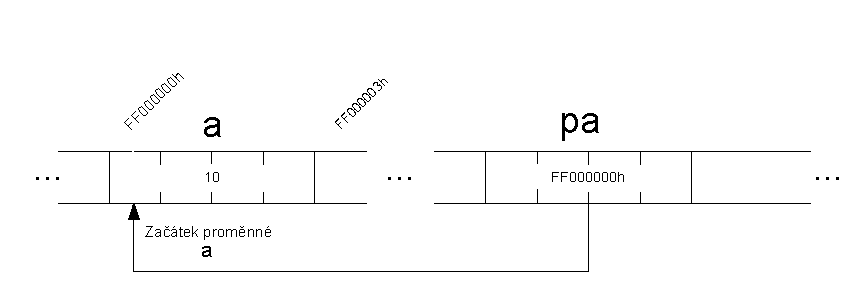
\includegraphics[width=0.9\linewidth]{princip_ukazatele.pdf}
        \caption{Princip ukazatele v paměti}
        \label{figure:pointer1}
      \end{figure}
      \begin{example}Vytvořte funkce kopírující prvky jednoho pole do druhého pomocí indexu i 
        ukazatele.
      
        % \marginpar{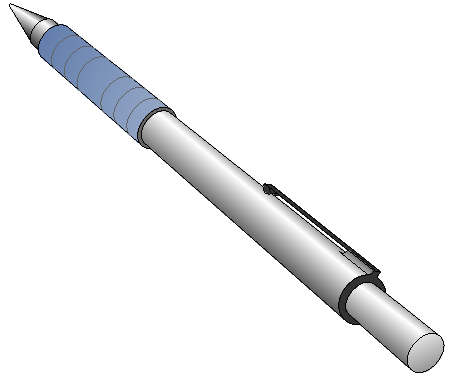
\includegraphics[width=0.09\textwidth]{pen.pdf}}
        %---------------------------------------------------------------
        \lstset{xrightmargin=13em}
        \lstinputlisting[caption=\texttt{CPYARRY.C} Kopíruje prvky jednoho pole do 
          druhého.]{../src/CES/C/CPYARRY.c}
        %---------------------------------------------------------------
       
       Výstup programu:%
       \begin{mdframed}[backgroundcolor=black, linecolor=white, %
                         fontcolor=white, userdefinedwidth=5cm, align=center, %
                         linecolor=gray, linewidth=3pt]
       \texttt{\textbf{1   2   3   4   5   6   7   8   9}} \\
       \texttt{\textbf{1   2   3   4   5   6}} \\
       \texttt{\textbf{4   5   6   7   8   9}}
       \end{mdframed} `
     \end{example}
  %============= Podkapitola: Preprocesor jazyka C =================================================
  \section{Preprocesor jazyka C}
    Preprocesor interpretuje jednoduché direktivy pro vložení zdrojového kódu z jiného souboru 
    (\lstinline[basicstyle=\ttfamily]!#include!), definice maker 
    (\lstinline[basicstyle=\ttfamily]!#define!) a podmíněné vložení kódu 
    (\lstinline[basicstyle=\ttfamily]!#if!). \texttt{C} preprocesor přijímá tyto direktivy:
    
    \begin{table}[ht!]
      \centering
      \begin{tabular}{c c c c}
        \hline
        \lstinline[basicstyle=\ttfamily]!#define!  & \lstinline[basicstyle=\ttfamily]!#elif! & 
        \lstinline[basicstyle=\ttfamily]!#else!    & \lstinline[basicstyle=\ttfamily]!#endif!  \\
        \lstinline[basicstyle=\ttfamily]!#error!   & \lstinline[basicstyle=\ttfamily]!#if! & 
        \lstinline[basicstyle=\ttfamily]!#ifdef!   & \lstinline[basicstyle=\ttfamily]!#ifndef! \\
        \lstinline[basicstyle=\ttfamily]!#include! & \lstinline[basicstyle=\ttfamily]!#line! & 
        \lstinline[basicstyle=\ttfamily]!#pragma!  & \lstinline[basicstyle=\ttfamily]!#undef!  \\
        \hline            
      \end{tabular}
      \caption{Seznam platných direktiv jazyka \texttt{C}}\label{S4101C1:C_tab_direktiva}
    \end{table} 
    
    \subsection{Připojení externích souborů}
    
    \subsection{Definice maker}
      Definice maker ve významu rozsahů polí je typickým příkladem použití preprocesoru. Ve 
      zdrojovém textu se neodvoláváme na magická čísla, ale na vhodně symbolicky pojmenovaná makra, 
      která zvýší čitelnost programu.
      
      Pro větší přehlednost rozdělme makra na 
      \begin{itemize}
       \item symbolické konstanty,
       \item makra
      \end{itemize}
      Klíčem nechť je skutečnost, že makro na rozdíl od symbolické konstanty má argumenty.
      \subsection{Symbolické konstanty}
      \subsection{Makra}
     
    \subsection{Podmíněný překlad}  
      Preprocesor může během své činnosti vyhodnocovat, je-li nějaké makro definováno, či nikoliv. 
      Při použití klíčového slova preprocesoru \texttt{defined} pak může spojovat taková 
      vyhodnocení do rozsáhlejších logických výrazů. Argument defined nemusí být uzavřen do 
      závorek. Může se však vyskytnout jen za \lstinline[basicstyle=\ttfamily]!#if! nebo 
      \lstinline[basicstyle=\ttfamily]!#elif!. Například si ukažme složitější podmínku:


  %============= Podkapitola: Terminálový vstup a výstup============================================
  \section{Terminálový vstup a výstup}
    Jazyk C, narozdíl od Pascalu, nedefinuje žádnou \texttt{I/O (vstup\-ně/výstup\-ní 
    -In\-put/Out\-put)} operaci jako část jazyka. Nezbytné vstupy a výstupy jsou řešeny tak, že 
    standardní knihovna obsahuje několik funkcí, které \texttt{I/O} zajišťují.
  
    Nejvíce strojově závislé akce jsou I/O operace a tímto způsobem se tedy důsledně oddělují 
    strojově závislé a strojově nezávislé části jazyka. Tato skutečnost je pak významným přínosem 
    při vytváření kompilátoru pro jiný počítač.
  
    \begin{figure}[ht!]
      \centering
      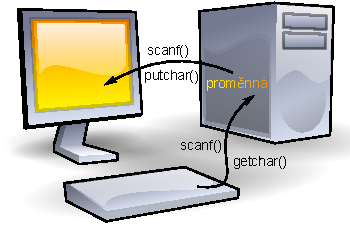
\includegraphics[scale=1.2]{terminalovy_IO_skica.pdf}
      \caption{Operace pro terminálový vstup a výstup}\label{C:fig_Terminal_IO}
    \end{figure}
  
    \subsection{Hlavičkový soubor \texttt{stdio.h}}
      Aby bylo možno správně používat všechny funkce pro vstupu a výstupu, je nutné na začátku 
      programu připojit "popis" těchto funkcí. Ten se nachází v hlavičkovém (\emph{header}) souboru 
      \lstinline[basicstyle=\ttfamily]!stdio.h!:
  
      \lstinline[basicstyle=\ttfamily]!#include <stdio.h>  //zde neni strednik!
  
      Od tohoto okamžiku je pak možné používat dále popsané funkce.
  
    \subsection{Standardní vstup a výstup znaku}
      Výstup jednoho znaku zajišťuje \lstinline[basicstyle=\ttfamily]!putchar()! a vstup jednoho 
      znaku funkce \lstinline[basicstyle=\ttfamily]!getchar()!.
      \begin{itemize}
        \item \lstinline[basicstyle=\ttfamily]!int putchar(int c);!
        \item \lstinline[basicstyle=\ttfamily]!int getchar(void);!
      \end{itemize}
      Obě funkce pracují s proměnnými \lstinline[basicstyle=\ttfamily]!int! a ne 
      \lstinline[basicstyle=\ttfamily]!char!.
  
        % \marginpar{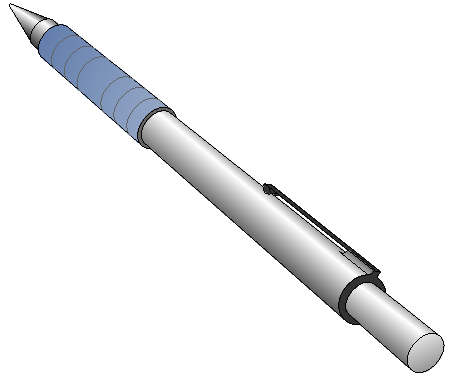
\includegraphics[width=0.09\textwidth]{pen.pdf}}
        %---------------------------------------------------------------
        \lstinputlisting[caption=\texttt{Cteni\_tisk\_znaku.c} Čtení a tisk znak ze 
           standardního vstupu na standardní výstup.]{../src/CES/C/Cteni_tisk_znaku.c} 
        %--------------------------------------------------------------    
      
      \begin{example}Čtení znaku ze standardního vstupu a jejich zápis na standardní výstup 
        ukazuje následující program, představující jednoduchou variantu příkazu kopírování souboru 
        (nutno ovšem přesměrovat vstup a výstup).
  
        % \marginpar{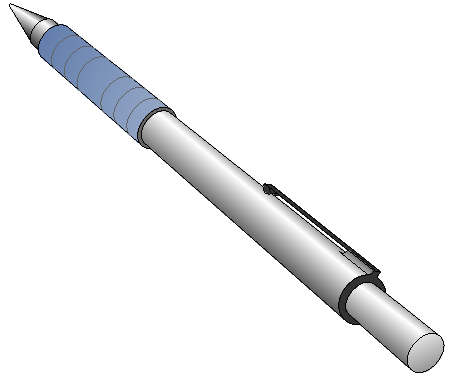
\includegraphics[width=0.09\textwidth]{pen.pdf}}
        %---------------------------------------------------------------
        \lstinputlisting[caption=\texttt{CPY.c} Kopíruje znak ze standardního vstupu na 
                standardní výstup.]{../src/CES/C/CPY.c}
        %---------------------------------------------------------------
      \end{example}
      
    \subsection{Standardní vstup a výstup řetězců}
      Standardní vstup a výstup řetězců je jednoduchou nadstavbou nad čtením znaku. Obě funkce,
      \begin{itemize}
        \item \lstinline[basicstyle=\ttfamily]!char *gets(char *s);!
        \item \lstinline[basicstyle=\ttfamily]!int puts(const char *s);!
      \end{itemize}
      pracují s řetězci. \texttt{gets()} načte do znakového pole vstupní řetězec az do konce řádku, 
      symbol  \lstinline[basicstyle=\ttfamily]!'\n'! není do znakového pole zapsán. Ukazatel na 
      pole (načtený řetězec) je rovněž návratovou hodnotou. Chybu signalizuje návrat NULL. 
      \texttt{puts()} 
      zapíše řetězec na výstup a přidá přechod na novy řádek       
      \lstinline[basicstyle=\ttfamily]!'\n'!. Chybu představuje návratové \texttt{EOF}, jinak vrací 
      kladné cele číslo.
  
      Jednoduchost použití skrývá velké nebezpečí. Funkce \texttt{gets()} nemá informaci o délce 
      oblasti vymezené pro čtený řetězec. Je-li oblast kratší, než vstupní řádek, dojde jeho 
      načtením velmi pravděpodobně k přepsání paměťové oblasti související s vyhrazenou pamětí. A 
      to se všemi důsledky z toho vyplývajícími.
  
    \subsection{Formátovaný standardní vstup a vystup}
    \subsection{Souhrnné cvičení}
      \begin{example}Vytvořte program, který vygeneruje ASCII tabulku se čtyřmi sloupci ve formátu 
      \textbf{[znak|kód|znak|kód]}. Rozsah tabulky definujte pomocí dvou symbolických konstant 
      \lstinline[basicstyle=\ttfamily]!MIN_ASCII, MAX_ASCII!. 
  
        % \marginpar{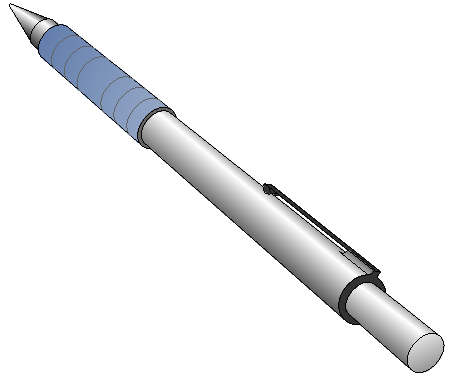
\includegraphics[width=0.09\textwidth]{pen.pdf}}
        %---------------------------------------------------------------
        \lstinputlisting[caption=\texttt{ASCII.c} Generuje ASCII tabulku na terminálu.]{../src/CES/C/ASCII.c}
        %---------------------------------------------------------------
      \end{example} 

%} % tikzset
%---------------------------------------------------------------------------------------------------
\printbibliography[title={Seznam literatury}, heading=subbibliography]
\addcontentsline{toc}{section}{Seznam literatury}